\documentclass{article}
\usepackage{graphicx}
\usepackage{titletoc}
\usepackage{titlesec}
\usepackage{geometry} 
\usepackage{fontspec, xunicode, xltxtra}
\usepackage{float}
\usepackage{cite}
\usepackage{amsmath}
\usepackage{listings}
\usepackage{titletoc}

\geometry{left=3cm,right=3cm,top=3cm,bottom=3cm}
\DeclareMathOperator*{\argmin}{argmin}
\DeclareMathOperator*{\argmax}{argmax}
\DeclareMathOperator*{\logit}{logit}
\DeclareMathOperator*{\var}{var}
\DeclareMathOperator*{\cov}{cov}
\DeclareMathOperator*{\expec}{E}
\DeclareMathOperator*{\deriv}{d}
\DeclareMathOperator*{\const}{constant}

\begin{document}
\title{\textsf{Homework 4 for Bayesian Data Analysis}}
\author{Fan JIN\quad (2015011506)}
\maketitle

\section*{Question 5.10a}
{
    $$p(\mu, \tau | y) \propto p(\mu, \tau) p(y | \mu, \tau) = p(\mu, \tau) \cdot \prod_{j=1}^{J} {N(\bar{y}_{.j} | \mu, \sigma_j^2 + \tau^2)}$$
    $$\propto \tau^{-1} \cdot \prod_{j=1}^{J} {(\sigma_j^2 + \tau^2)^{-1/2} \exp{ \left( - \frac{(\bar{y}_{.j} - \mu)^2}{2(\sigma_j^2 + \tau^2)} \right) }},$$
    where $\sigma_j^2 = \sigma^2 / n_j$ is the variance of the $j$-th group.

    As $\tau \rightarrow 0$, the posterior pdf $p(\mu, \tau | y)$ is dominated by $\tau^{-1}$, which is not integrable. Therefore, the posterior distribution is improper.
}

\section*{Question 5.10b}
{
    $$p(\mu, \tau | y) \propto p(\mu, \tau) p(y | \mu, \tau) = p(\mu, \tau) \cdot \prod_{j=1}^{J} {N(\bar{y}_{.j} | \mu, \sigma_j^2 + \tau^2)}$$
    $$= \prod_{j=1}^{J} {(\sigma_j^2 + \tau^2)^{-1/2} \exp{ \left( - \frac{(\bar{y}_{.j} - \mu)^2}{2(\sigma_j^2 + \tau^2)} \right) }}$$
    $$= \left[ \prod_{j=1}^{J} {(\sigma_j^2 + \tau^2)} \right]^{-1/2} \cdot \exp{\left[ -\frac{1}{2} \sum_{j=1}^{J} {\frac{(\bar{y}_{.j} - \mu)^2}{\sigma_j^2 + \tau^2}} \right]}$$
    $$= \left[ \prod_{j=1}^{J} {(\sigma_j^2 + \tau^2)} \right]^{-1/2} \cdot \exp{\left[ -\frac{1}{2} {\left( A(\mu-B)^2 + C \right)} \right]}$$
    $$= \left[ \prod_{j=1}^{J} {(\sigma_j^2 + \tau^2)} \right]^{-1/2} \cdot \exp{\left[ -\frac{A}{2} (\mu-B)^2 \right]} \cdot \exp{(-\frac{C}{2})},$$
    where $$A = \sum_{j=1}^{J} {\frac{1}{(\sigma_j^2 + \tau^2)}},$$
    $$C = \left[ \sum_{j=1}^{J} {\frac{\bar{y}_{.j}^2}{(\sigma_j^2 + \tau^2)}} \right] - A^{-1} \left[ \sum_{j=1}^{J} {\frac{\bar{y}_{.j}}{(\sigma_j^2 + \tau^2)}} \right]^2 .$$

    It follows that 
    $$\int_{-\infty}^{\infty} {p(\mu, \tau | y) \deriv{\mu}} \propto \left[ \prod_{j=1}^{J} {(\sigma_j^2 + \tau^2)} \right]^{-1/2} \cdot A^{-1/2} \cdot \exp{(-\frac{C}{2})}.$$

    As $\tau \rightarrow 0$, the integral above goes to a finite constant. As $\tau \rightarrow \infty$, we have
    $$A \rightarrow J \tau^{-2},$$
    $$C \rightarrow \tau^{-2} \cdot \left[ \sum_{j=1}^{J}{\bar{y}_{.j}^2} - \frac{1}{J} (\sum_{j=1}^{J}{\bar{y}_{.j}})^2 \right],$$
    and the integral above is therefore dominated by
    $$\tau^{-J} \cdot J^{-1/2} \tau \cdot \exp{\left(-\frac{D}{2} \tau^{-2}\right)} \propto \tau^{-(J-1)} \exp{\left(-\frac{D}{2} \tau^{-2}\right)} \rightarrow \tau^{-(J-1)},$$ 
    where $$D = \sum_{j=1}^{J}{\bar{y}_{.j}^2} - \frac{1}{J} (\sum_{j=1}^{J}{\bar{y}_{.j}})^2 > 0.$$
    Since $\tau^{-(J-1)}$ is integrable with respect to $\tau$ if $J > 2$, the posterior distribution is proper:
    $$\int_{0}^{\infty} { \left\{ \int_{-\infty}^{\infty} {p(\mu, \tau | y) \deriv{\mu}} \right\} \deriv{\tau}} < \infty.$$
}

\section*{Question 5.10c}
{
    We don't have enough information to infer if we only have two groups in the hierarchical model, as the hyperparameters $(\mu, \tau)$ is estimated precisely when $J$ is large. So it is an alternative to use a model other than hierarchical model, e.g., to assume the two schools are independent of each other, and assign independent prior distribution for each school (i.e. treat the two schools separately), as shown below:
    $$y_{1j} \sim^{\mathrm{i.i.d.}} N(\theta_1, \sigma^2), \quad y_{2j} \sim^{\mathrm{i.i.d.}} N(\theta_2, \sigma^2),$$
    where $\sigma^2$ is known, and $$\theta_1 \sim N(\mu_1, \tau_1^2), \quad \theta_2 \sim N(\mu_2, \tau_2^2)$$ with hyperparameters $(\mu_1, \mu_2, \tau_1, \tau_2)$. Thus, $p(\mu_1, \tau_1 | \bar{y}_{1j})$ and $p(\mu_2, \tau_2 | \bar{y}_{2j})$ can be obtained separately.

}

\section*{Question 5.12}
{
    First, we have
    $$\theta_j | \mu, \tau, y \sim N( \frac{\frac{1}{\sigma_j^2} \bar{y}_{.j} + \frac{1}{\tau^2} \mu}{\frac{1}{\sigma_j^2} + \frac{1}{\tau^2}}, \frac{1}{\frac{1}{\sigma_j^2} + \frac{1}{\tau^2}}).$$
    It follows that $$\expec{(\theta_j | \mu, \tau, y)} = \frac{\frac{1}{\sigma_j^2} \bar{y}_{.j} + \frac{1}{\tau^2} \mu}{\frac{1}{\sigma_j^2} + \frac{1}{\tau^2}},$$
    $$\var{(\theta_j | \mu, \tau, y)} = \frac{1}{\frac{1}{\sigma_j^2} + \frac{1}{\tau^2}}.$$

    Second, we have
    $$\mu | \tau, y \sim N( \frac{\sum_{j=1}^{J}{\frac{1}{\sigma_j^2+\tau^2} \bar{y}_{.j}}}{\sum_{j=1}^{J}{\frac{1}{\sigma_j^2+\tau^2}}}, \left( \sum_{j=1}^{j}{\frac{1}{\sigma_j^2+\tau^2}} \right)^{-1} ).$$
    It follows that $$\expec{(\mu | \tau, y)} = \frac{\sum_{j=1}^{J}{\frac{1}{\sigma_j^2+\tau^2} \bar{y}_{.j}}}{\sum_{j=1}^{J}{\frac{1}{\sigma_j^2+\tau^2}}},$$
    $$\var{(\mu | \tau, y)} = (\sum_{j=1}^{j}{\frac{1}{\sigma_j^2+\tau^2}})^{-1}.$$

    Therefore, the posterior expectation and variance of $\theta_j$ conditional on $\tau$ and $y$ are:
    $$\expec{(\theta_j | \tau, y)} = \expec_{\mu | \tau, y}{\left[ \expec{(\theta_j | \mu, \tau, y)} \right]} $$
    $$= \expec_{\mu | \tau, y}{\left[ \frac{\frac{1}{\sigma_j^2} \bar{y}_{.j} + \frac{1}{\tau^2} \mu}{\frac{1}{\sigma_j^2} + \frac{1}{\tau^2}} \right]}$$
    $$= \frac{\frac{1}{\sigma_j^2} \bar{y}_{.j} + \frac{1}{\tau^2} \expec{(\mu | \tau, y)}}{\frac{1}{\sigma_j^2} + \frac{1}{\tau^2}}$$
    $$= \frac{\frac{1}{\sigma_j^2} \bar{y}_{.j} + \frac{1}{\tau^2} \frac{\sum_{j=1}^{J}{\frac{1}{\sigma_j^2+\tau^2} \bar{y}_{.j}}}{\sum_{j=1}^{J}{\frac{1}{\sigma_j^2+\tau^2}}}}{\frac{1}{\sigma_j^2} + \frac{1}{\tau^2}},$$
    and
    $$\var{(\theta_j | \tau, y)} = \expec_{\mu | \tau, y}{\left[ \var{(\theta_j | \mu, \tau, y)} \right]} + \var_{\mu | \tau, y}{\left[ \expec{(\theta_j | \mu, \tau, y)} \right]}$$
    $$= \frac{1}{\frac{1}{\sigma_j^2} + \frac{1}{\tau^2}} + \var_{\mu | \tau, y}{\left[ \frac{\frac{1}{\sigma_j^2} \bar{y}_{.j} + \frac{1}{\tau^2} \mu}{\frac{1}{\sigma_j^2} + \frac{1}{\tau^2}} \right]}$$
    $$= \frac{1}{\frac{1}{\sigma_j^2} + \frac{1}{\tau^2}} + \left( \frac{\frac{1}{\tau^2}}{\frac{1}{\sigma_j^2} + \frac{1}{\tau^2}} \right)^2 \var{(\mu | \tau, y)}$$
    $$= \frac{1}{\frac{1}{\sigma_j^2} + \frac{1}{\tau^2}} + \left( \frac{\frac{1}{\tau^2}}{\frac{1}{\sigma_j^2} + \frac{1}{\tau^2}} \right)^2 (\sum_{j=1}^{j}{\frac{1}{\sigma_j^2+\tau^2}})^{-1}$$

}

\section*{Question 5.15a}
{
    Build the hierarchical model below:
    $$y_j | \theta_j, \sigma_j \sim N(\theta_j, \sigma_j^2),$$
    where $$y_j = \logit{(y_{1j} / n_{1j})} - \logit{(y_{0j} / n_{0j})}$$ is the log-odds (observed data), and $$\sigma_j^2 = (y_{1j})^{-1} + (n_{1j} - y_{1j})^{-1} + (y_{0j})^{-1} + (n_{0j} - y_{0j})^{-1}$$ is the approximated sampling variance (assumed known). And the model paramters $$\theta_j \sim^{\mathrm{i.i.d.}} N(\mu, \tau^2)$$ with hyperparameters $(\mu, \tau)$.

    Assign a noninformative hyperprior distribution $p(\mu, \tau) \propto 1$. It follows from Question 5.10b that
    $$p(\tau | y) = \int_{-\infty}^{\infty} {p(\mu, \tau | y) \deriv{\mu}} \propto \left[ \prod_{j=1}^{J} {(\sigma_j^2 + \tau^2)} \right]^{-1/2} \cdot A^{-1/2} \cdot \exp{(-\frac{C}{2})},$$ where $A$, $C$ are defined in my answer to Question 5.10b:
    $$A = \sum_{j=1}^{J} {\frac{1}{(\sigma_j^2 + \tau^2)}},$$
    $$C = \left[ \sum_{j=1}^{J} {\frac{\bar{y}_{.j}^2}{(\sigma_j^2 + \tau^2)}} \right] - A^{-1} \left[ \sum_{j=1}^{J} {\frac{\bar{y}_{.j}}{(\sigma_j^2 + \tau^2)}} \right]^2 .$$

    Although the expression is a bit complicated for analysis, it can be easily calculated numerically. Below is the output in R:
    \begin{figure}[H]
        \centering
        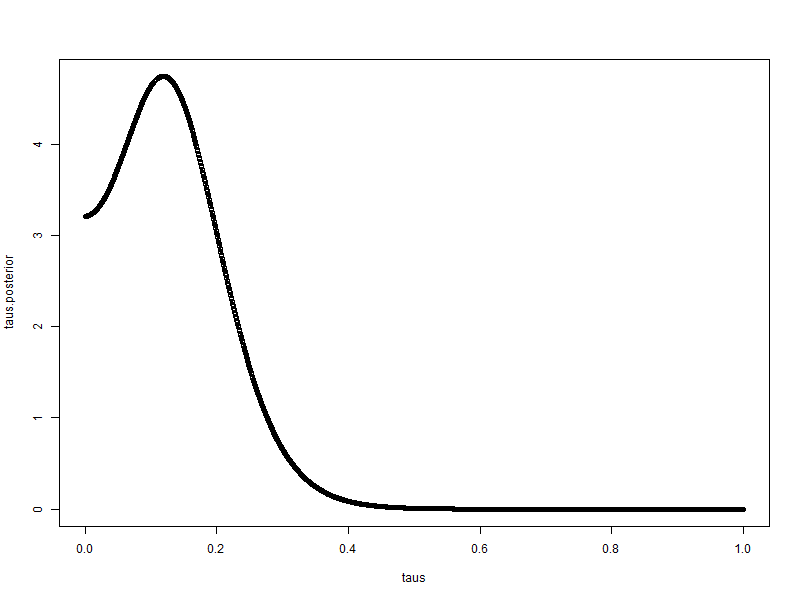
\includegraphics[width = 0.8\linewidth]{tau.posterior.png}
        \caption{Posterior density of $\tau$}
    \end{figure}

}

\section*{Question 5.15b}
{
    Based on what we obtained in Question 5.12 about the posterior mean and variance of $\theta_j$ conditional on $\tau$, we get the plots below. 
    \begin{figure}[H]
        \centering
        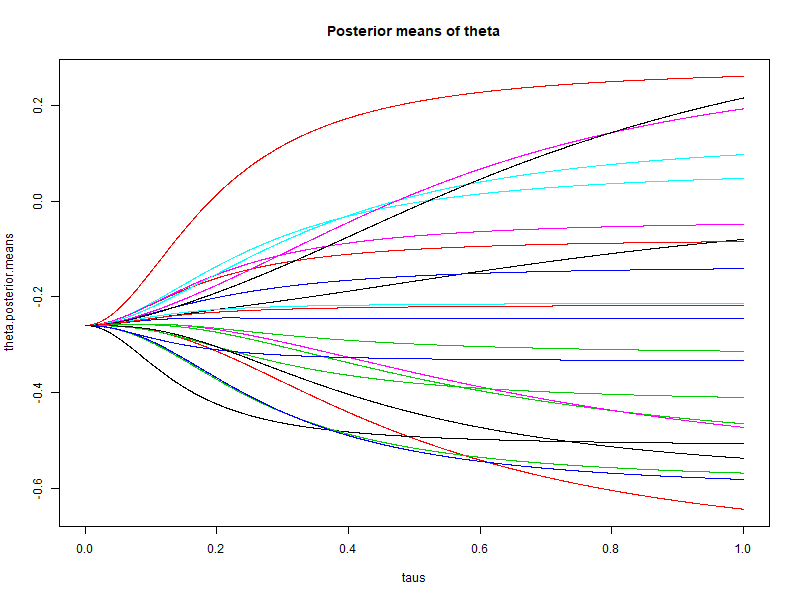
\includegraphics[width = 1.0\linewidth]{theta.posterior.means.png}
        \caption{Posterior means of $\theta_j$}
    \end{figure}
    \begin{figure}[H]
        \centering
        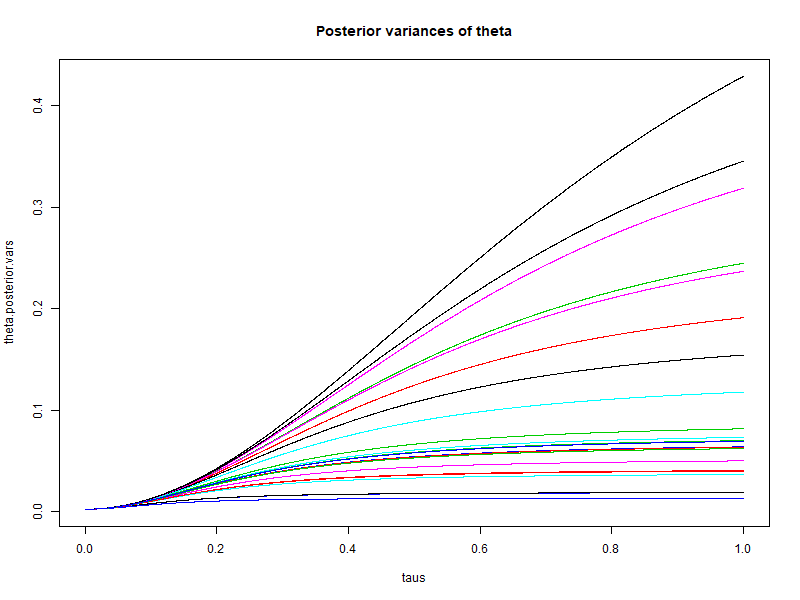
\includegraphics[width = 1.0\linewidth]{theta.posterior.vars.png}
        \caption{Posterior variances of $\theta_j$}
    \end{figure}
    
}

\section*{Question 5.15c}
{
    First, we obtained the posterior joint distribution for hyperparameters in Question 5.10b:
    $$p(\mu, \tau | y) \propto \left[ \prod_{j=1}^{J} {(\sigma_j^2 + \tau^2)} \right]^{-1/2} \cdot \exp{\left[ -\frac{A}{2} (\mu-B)^2 \right]} \cdot \exp{(-\frac{C}{2})},$$
    where $$A = \sum_{j=1}^{J} {\frac{1}{(\sigma_j^2 + \tau^2)}},$$
    $$C = \left[ \sum_{j=1}^{J} {\frac{\bar{y}_{.j}^2}{(\sigma_j^2 + \tau^2)}} \right] - A^{-1} \left[ \sum_{j=1}^{J} {\frac{\bar{y}_{.j}}{(\sigma_j^2 + \tau^2)}} \right]^2 .$$

    Second, we have 
    $$p(\theta_j | \mu, \tau, y) \propto (V_j)^{-1/2} \exp{(-\frac{(\theta_j - \hat{\theta}_j)^2}{2V_j})}, $$
    where $$\hat{\theta}_j = \frac{\frac{1}{\sigma_j^2} \bar{y}_{.j} + \frac{1}{\tau^2} \mu}{\frac{1}{\sigma_j^2} + \frac{1}{\tau^2}}, $$
    $$V_j = \left( \frac{1}{\sigma_j^2} + \frac{1}{\tau^2} \right)^{-1}.$$

    It follows that 
    $$p(\theta_j | y) = \int_{0}^{\infty} {\int_{-\infty}^{\infty} {p(\mu, \tau | y) \cdot p(\theta_j | \mu, \tau, y) \deriv{\mu}} \deriv{\tau}}.$$ The median of $\theta_j | y$ is obtained as well.
}

\section*{Question 5.15d}
{
    First, draw $\tau$ from $p(\tau | y)$. Then draw $\mu$ from $p(\mu | \tau, y)$. Finally, draw $\theta_j$ from $p(\theta_j | \mu, \tau, y)$.

    \begin{figure}[H]
        \centering
        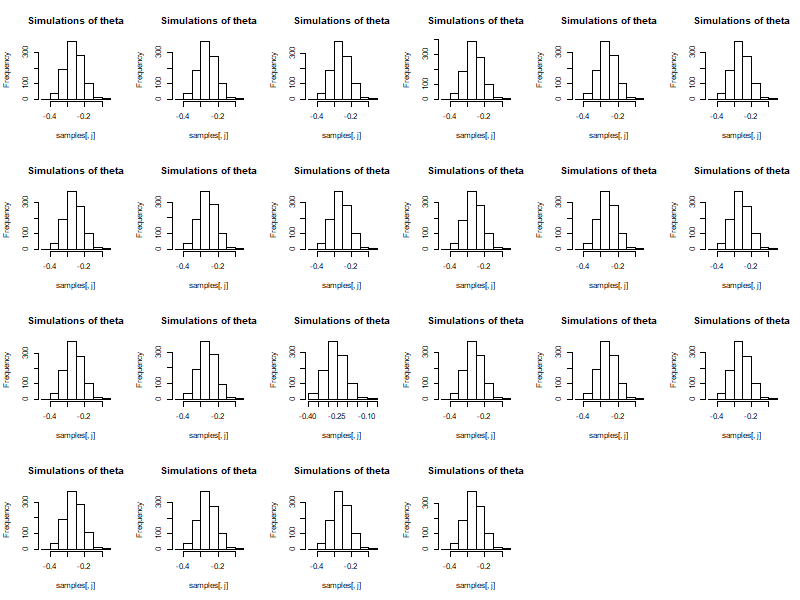
\includegraphics[width = 1.0\linewidth]{theta.simulations.png}
        \caption{Simulations of $\theta_j$s}
    \end{figure}
}

\section*{Question 5.15e}
{
    I failed to simulate $y_{1j}$ and $y_{0j}$ from the $\theta_j$s simulated in Question 5.15d, because we cannot obtain the likelihood $$p(y_j | \theta_j, \sigma_j^2) = N(\theta_j, \sigma_j^2)$$ with $\sigma_j^2$ unknown for the hypothetical new study, although $\theta_j$ has been simulated in Question 5.15d.
}

\section*{Source Code in R:}
{
    Raw file: http://39.106.23.58/files/BayesianHW4.7z

    \begin{lstlisting}[language=R]
        plot.increment = 0.0005
        dat = read.csv("data.csv", header=T)
        
        logit <- function(x) {
          return (log(x / (1 - x)))
        }
        
        log.odds = logit(dat$treated.deaths / dat$treated.total) - logit(dat$control.deaths / dat$control.total)
        std.err = sqrt((dat$treated.deaths)^(-1) + 
                         (dat$treated.total - dat$treated.deaths)^(-1) + 
                         (dat$control.deaths)^(-1) +
                         (dat$control.total - dat$control.deaths)^(-1))
        
        dat = cbind(dat, log.odds)
        dat = cbind(dat, std.err)
        
        J = nrow(dat)
        
        # Question 5.15a
        
        tau.posterior <- function(tau, dat) {
          J = nrow(dat)
          
          A = 0
          for (j in 1:J) {
            A = A + 1 / (dat$std.err[j]^2 + tau^2)
          }
          
          S1 = 0
          for (j in 1:J) {
            S1 = S1 + (dat$log.odds[j]) / (dat$std.err[j]^2 + tau^2)
          }
          
          S2 = 0
          for (j in 1:J) {
            S2 = S2 + (dat$log.odds[j]^2) / (dat$std.err[j]^2 + tau^2)
          }
          
          C = S2 - S1^2 / A
          
          P = 0
          for (j in 1:J) {
            P = P + (-1/2) * log(dat$std.err[j]^2 + tau^2)
          }
          P = exp(P)
          
          return (P * A^(-1/2) * exp(-C/2))
          
        }
        
        taus = seq(0 + plot.increment, 1, by = plot.increment)
        taus.posterior = unlist(lapply(taus, tau.posterior, dat))
        taus.posterior = taus.posterior / sum(taus.posterior) / plot.increment # rescale to 1
        
        png("tau.posterior.png", width = 800, height = 600)
        plot(taus, taus.posterior)
        dev.off()
        
        # Question 5.15b
        
        theta.posterior.mean <- function(tau, dat) {
          J = nrow(dat)
          
          S0 = 0
          for (j in 1:J) {
            S0 = S0 + 1 / (dat$std.err[j]^2 + tau^2)
          }
          
          S1 = 0
          for (j in 1:J) {
            S1 = S1 + (dat$log.odds[j]) / (dat$std.err[j]^2 + tau^2)
          }
          
          ret = 1:12
          for (j in 1:J) {
            A = dat$log.odds[j] / dat$std.err[j]^2 + 1 / tau^2 * S1 / S0
            B = 1 / dat$std.err[j]^2 + 1 / tau^2
            ret[j] = A / B
          }
          
          return (ret)
        }
        
        theta.posterior.var <- function(tau, dat) {
          J = nrow(dat)
          
          S0 = 0
          for (j in 1:J) {
            S0 = S0 + 1 / (dat$std.err[j]^2 + tau^2)
          }
          
          ret = 1:12
          for (j in 1:J) {
            A = 1 / tau^2
            B = 1 / dat$std.err[j]^2 + 1 / tau^2
            ret[j] = 1 / B + (A / B)^2 / S0
          }
          
          return (ret)
        }
        
        theta.posterior.means = lapply(taus, theta.posterior.mean, dat)
        theta.posterior.means = matrix(unlist(theta.posterior.means), ncol=J, byrow=T)
        
        theta.posterior.vars = lapply(taus, theta.posterior.var, dat)
        theta.posterior.vars = matrix(unlist(theta.posterior.vars), ncol=J, byrow=T)
        
        png("theta.posterior.means.png", width = 800, height = 600)
        matplot(taus, theta.posterior.means, type="l", lty=1, main="Posterior means of theta")
        dev.off()
        
        png("theta.posterior.vars.png", width = 800, height = 600)
        matplot(taus, theta.posterior.vars, type="l", lty=1, main="Posterior variances of theta")
        dev.off()
        
        # Question 5.15c
        
        index.MLE = which.max(taus.posterior) # use MLE of tau for a crude estimate of theta_j
        tau.MLE = taus[index.MLE]
        
        # Question 5.15d
        
        p.mu.tau.c.dat <- function(mu, tau, dat) {
          J = nrow(dat)
          
          A = 0
          for (j in 1:J) {
            A = A + 1 / (dat$std.err[j]^2 + tau^2)
          }
          
          S1 = 0
          for (j in 1:J) {
            S1 = S1 + (dat$log.odds[j]) / (dat$std.err[j]^2 + tau^2)
          }
          
          S2 = 0
          for (j in 1:J) {
            S2 = S2 + (dat$log.odds[j]^2) / (dat$std.err[j]^2 + tau^2)
          }
          
          C = S2 - S1^2 / A
          
          S3 = 0
          for (j in 1:J) {
            S3 = S3 + (dat$log.odds[j]) / (dat$std.err[j]^2 + tau^2)
          }
          
          B = S3 / A
          
          P = 0
          for (j in 1:J) {
            P = P + (-1/2) * log(dat$std.err[j]^2 + tau^2)
          }
          P = exp(P)
          
          return (P * exp(-A/2 * (mu - B)^2) * exp(-C/2))
        }
        
        p.theta.c.mu.tau.dat <- function(j, theta.j, mu, tau, dat) {
          J = nrow(dat)
          
          A = 1 / dat$std.err[j]^2
          B = 1 / tau^2
          
          theta.j.hat = (A * dat$log.odds[j] + B * mu) / (A + B)
          V.j = 1 / (A + B)
          
          return (V.j^(-1/2) * exp(-1/2 * (theta.j - theta.j.hat)^2 / V.j))
        }
        
        # Question 5.15d
        
        T = 1000
        samples = matrix(NA, T, J)
        
        for (k in 1:1000) {
          U = runif(1)
          temp = 1:length(taus)
          temp[1] = taus.posterior[1]
          V = 0
          for (j in 2:length(taus)) {
            temp[j] = temp[j - 1] + taus.posterior[j]
            if (temp[j] > U) {
              tau.sampled = taus[j] # sample tau
              break;
            }
          }
          
          J = nrow(dat)
          A = 0
          for (j in 1:J) {
            A = A + 1 / (dat$std.err[j]^2 + tau.sampled^2)
          }
          S3 = 0
          for (j in 1:J) {
            S3 = S3 + (dat$log.odds[j]) / (dat$std.err[j]^2 + tau.sampled^2)
          }
          B = S3 / A
          mu.sampled = rnorm(1, mean = B, sd = 1 / sqrt(A)) # sample mu
          
          J = nrow(dat)
          for (j in 1:J) {
            C = 1 / dat$std.err[j]^2
            D = 1 / tau.sampled^2
            
            theta.j.hat = (C * dat$log.odds[j] + D * mu.sampled) / (C + D)
            V.j = 1 / (C + D)
            theta.j.sampled = rnorm(1, theta.j.hat, sqrt(V.j)) # sample theta_j
            
            samples[k, j] = theta.j.sampled
          }
        }
        
        png("theta.simulations.png", width = 800, height = 600)
        par(mfrow=c(4,6))
        for (j in 1:J) {
          hist(samples[, j], main="Simulations of theta", pch = j)
        }
        dev.off()

    \end{lstlisting}
}

\clearpage
\end{document}
